\chapter{Réalisations}
%Si besoin, vous pourriez structurer le reste du rapport en plusieurs parties et non une seule. La ou les parties devraient elles-mêmes êtres structurées en plusieurs sous-sections au sein d'une même partie. Dans tous les cas, la logique du plan doit apparaître clairement.

%Travaillez les liaisons pour aboutir à une lecture fluide. Voici un exemple (un peu exagéré) : "Après avoir inventorié les technologies disponibles dans la section précédente, cette section est consacrée aux expérimentations que nous avons menées avec chacune d'elles. Ce travail nous permettra de sélectionner les technologies retenues, présentées dans la section suivante."

%Présentez votre réflexion et vos choix, qui devraient être justifiés. Examinez rapidement les autres alternatives.

%Sélectionnez les détails pertinents et laissez les autres en annexe. Allez du général au particulier. Evitez de présenter un catalogue des fonctions développées.
Le sujet de mon stage étant large, très tôt j'ai dû me concentrer sur plusieurs tâches puis rapidement m'atteler à plusieurs réalisations afin d'assurer au mieux ma fonction. Nous verrons donc dans ce chapitre, pour chacune de ces différentes réalisations, les besoins auxquels il fallait répondre, les choix qui ont été faits et les différentes difficultés rencontrées.

\section{Conception d'un processus de production et de gestion des rapports de test}
%QQchose ?
\subsection{État des lieux}
Dans un premier temps, une présentation du contexte initial est indispensable. Au sein de l'équipe \gls{TC}, il existe différentes phases de test, dont l'organisation correspond au cycle en V du projet (cf. Annexe I) :
\begin{itemize}
\item \textbf{FAT} : Factory Acceptance Test, test d'acceptation usine consistant à inspecter le système dans l'usine avant livraison. Pendant le FAT, les performances du système sont contrôlées, généralement en collaboration avec le client.
\item \textbf{iFAT} : Integrated Factory Acceptance Test, test d'acceptation intégré usine consistant à contrôler le fonctionnement des différents équipements ensemble.
\item \textbf{\gls{StAT}} : Stand Alone Test, test unitaire, où  l'équipement testé est isolé de toute interaction durant le test, afin de restreindre les critères du test à son fonctionnement autonome.
\item \textbf{\gls{SIT}} : Site Integration Test, test d'intégration, ayant pour but de détecter les erreurs non détectables pendant les tests unitaires. Ce type de test consiste à assembler différents composants afin de tester leur fonctionnement dans l'ensemble.
\item \textbf{\gls{E2E}} : End to End Test, test bout en bout ayant pour but de vérifier si un système se comporte comme prévu du début à la fin. Le testeur doit se mettre dans le rôle d’un utilisateur et effectuer les tests comme s’il utilisait véritablement l’outil mis à sa disposition.
\end{itemize}

Nous nous concentrerons ici sur les phases \gls{StAT}, \gls{SIT}, \gls{E2E}.

Pour chaque sous-système du projet, 3 procédures de test ont été rédigées, une par phase de test.

Ainsi, si une localisation du projet abrite 3 sous-systèmes nécessitant d'être testés, il y aura 9 tests à effectuer dans cette localisation.

Ensuite, chaque test doit être formalisé par un rapport de test constitué de la manière suivante :

\begin{itemize}
\item Une première page que l'on appelle ITR, qui permet d'identifier le rapport (numéro unique), d'identifier le test (localisation, phase, système, date), identifier le statut (accepté avec, sans réserve ou refusé), résumer les observations et réserves des 3 parties et consigner leurs signatures.
\item Les pages suivantes sont les \gls{TestCases}, en français les scénarios de test, qui permettent de simuler plusieurs situations d'utilisation des systèmes de manière à prouver leur conformité vis-à-vis de toutes les exigences du cahier des charges.
\begin{itemize}
\item Chaque \gls{TestCases} est composé de une ou plusieurs étapes qui elles-mêmes sont reliées à une ou plusieurs exigences.
\end{itemize}
\end{itemize}

Parmi ces exigences, certaines sont liées à la sécurité, dans le cadre des \gls{RAMS}, et sont indexées dans un document appelé le \gls{SC}. Ces exigences liées à la sécurité sont séparées en deux \gls{SIL}, ou niveaux de criticité : SIL0, le plus faible et SIL2 le plus élevé.

Une fois ce contexte clarifié, nous avons pu entreprendre l'élaboration du processus et c'est le sujet de la prochaine section.

\subsection{Première version}

Après l'analyse exposée précédemment, nous avons travaillé conjointement avec mon maître de stage sur une première version du processus que voici :

\begin{center}
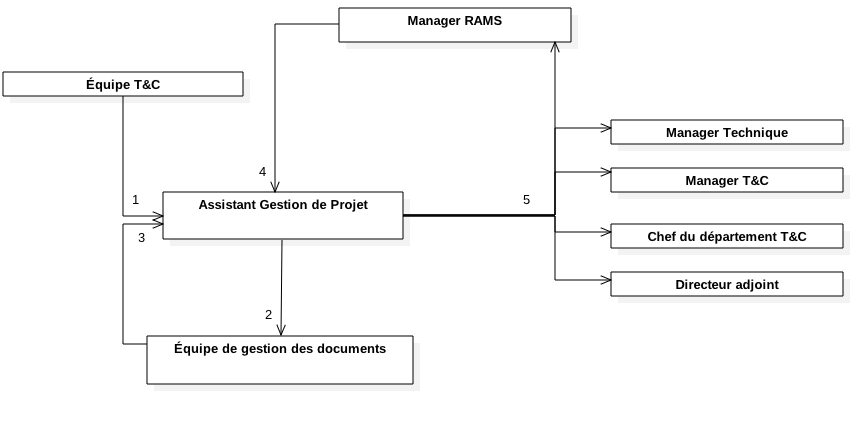
\includegraphics[height=7cm]{ressources/images/figures/Workflow1.png}
\end{center}


\begin{itemize}
\item \textbf{1.} Tout d'abord, l'équipe \gls{TC} effectue les différentes inspections et produit les rapports de test en remplissant les formulaires correspondant sur \gls{SnagR}.
\item \textbf{2.} Ensuite j'extraie les données de \gls{SnagR} (nous reviendrons sur ce point dans la prochaine partie) et les importe dans un fichier Excel afin de les exploiter. J'exporte les rapports au format PDF et les envoie à l'équipe de gestion des documents.
\item \textbf{3.} Cette dernière importe les rapports sur \gls{Mezzoteam} afin de rendre ces preuves accessibles à tous les membres du projet et les importe aussi sur \gls{e-TOL} pour que les membres de l'équipe Thales offshore puissent les consulter. Une fois l'importation terminée, l'équipe me fournit les références de ces documents afin que je les ajoute à ma base de données.
\item \textbf{4.} Le manager \gls{RAMS} et son équipe me fournissent des mises à jour concernant les exigences liées à la sécurité afin que je puisse actualiser mon fichier, car les rapports devant servir de preuve pour ces dernières nécessitent d'être suivis de manière prioritaire. En effet, le futur opérateur refusera de commencer la période de formation de ses employés à l'exploitation du système tant qu'il n'aura pas la preuve de la conformité du projet vis-à-vis de ces exigences.
\item \textbf{5.} Enfin, il me faut communiquer les résultats aux différents managers sous forme de \gls{KPI}, courbes et outils d'aide à la décision. Nous reviendrons plus tard sur ce point.
\end{itemize}

Ce processus fut mis en place et appliqué durant le premier mois de mon stage, mais il fallut rapidement l'adapter.

\subsection{Évolution du processus}

En effet, aux vues des différentes responsabilités que l'on m'a confiées à partir du second mois, j'ai dû intégrer à ce processus de nouvelles étapes.
Voici ci-dessous la matrice de responsabilité de notre projet suivant la méthode RACI. Dans cette matrice, le R signifie responsable et désigne la personne qui exécute l'action, le A désigne la personne qui approuve l'action, le C une personne consultée et le I une personne devant être tenue informée.

\begin{center}
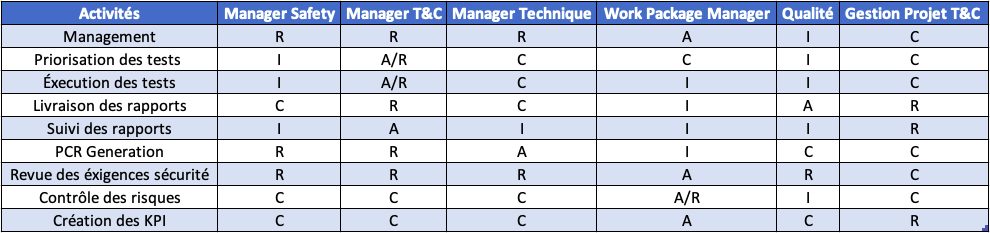
\includegraphics[height=4cm]{ressources/images/figures/RACI.png}
\end{center}

Ainsi, c'est pour cela que j'ai dû choisir d'intégrer au processus de nouveaux acteurs ainsi que de nouvelles interactions.

\begin{center}
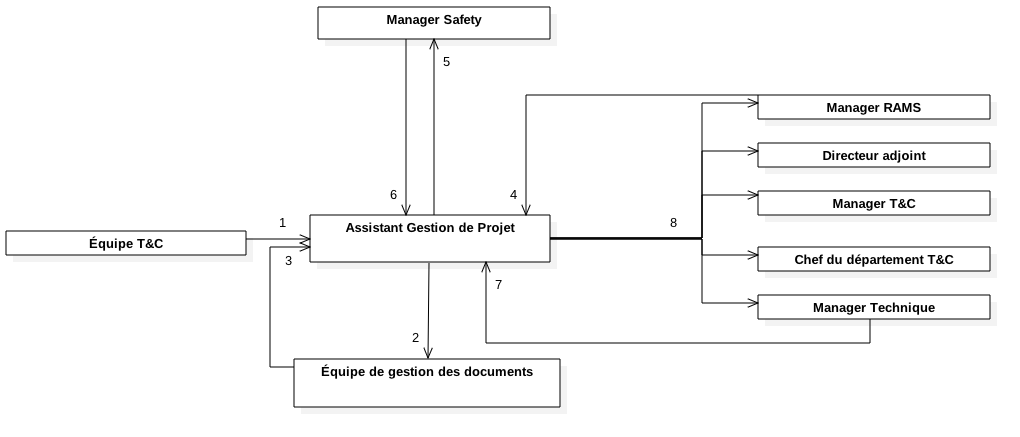
\includegraphics[height=7cm]{ressources/images/figures/Workflow2.png}
\end{center}


\begin{itemize}
\item \textbf{Étapes 1 à 4.} Identiques à la première version du processus.
\item \textbf{5.} Après avoir vérifié que les exigences liées à la sécurité étaient bien à jour, il me fallait fournir au manager sécurité les données nécessaires à la vérification de la conformité des systèmes. Je devais donc lui fournir, pour chaque exigence déjà vérifiée lors d'un test, la référence du rapport de ce test ainsi que celles des \gls{TestCases} permettant de vérifier la conformité de l'exigence.
\item \textbf{6.} Ensuite, le manager sécurité devait spécifier, pour chaque \gls{TestCases} lié à une exigence sécurité, si il était conforme ou non, et le cas échéant, il devait générer une \gls{PCR} afin de notifier ce défaut aux autres équipes.
\item \textbf{7.} Après cela, je collectais, auprès du manager technique (et de son équipe), les différents facteurs limitants retardant l'exécution de certains tests, afin de pouvoir, à l'étape suivante, réaliser des outils d'aide à la décision.
\item \textbf{8.} Comme précédemment, il fallait enfin communiquer les résultats aux managers.
\end{itemize}

Dans un souci de synthèse, la version du processus final exposée ci-dessus est une version simplifiée, mais les étapes principales y sont représentées.
Au cours de la prochaine partie, nous allons nous intéresser à la réalisation de la deuxième étape du processus : l'extraction des données.

\newpage
\section{Mise au point d'un outil d'extraction de données }
%QQchose ?
Cette partie constitue le point névralgique du processus, car sans données, aucune des étapes suivantes n'est réalisable. Mais c'est aussi le point le plus complexe et c'est pour cela que cette réalisation fut la plus conséquente de mon stage.
\subsection{Les motivations}
Au tout début de mon stage, je me chargeais de l'extraction de ces données manuellement, puisque le nombre de rapports de test remplis était réduit.

Mais rapidement il fallut envisager une alternative, car sur cette phase du projet, environ 1500 rapports de test seraient produits, soit plus de 15 000 \gls{TestCases} (donc autant de formulaires), soit plus de 60 000 étapes de test à analyser.

De plus, le contenu de ces rapports de test étant dynamique (puisque les utilisateurs de \gls{SnagR} pouvaient éditer le même rapport à maintes reprises), il aurait fallu actualiser cette énorme quantité de données régulièrement.

Ainsi, j'ai essayé, en demandant au client des droits d'accès plus élevés sur \gls{SnagR}, d'obtenir les données automatiquement en utilisant les fonctions proposées par l'outil.

Mais ces fonctions d'exportation de données présentaient deux défauts majeurs :
\begin{itemize}
\item Les champs et les différents lots de données proposés au moment de l'exportation étaient trop restreints, il n'était pas possible d'exporter toutes les données issues des rapports.
\item Les données étaient structurées autour d'un découpage basé sur des activités, pour faire simple, ce dernier ne correspondait pas au découpage énoncé précédemment : 1 rapport par localisation pour chaque type de test et pour chaque système. Les données manquaient de cohérence, le nombre total d'activités étant de 6000 alors que seules 1500 de ces activités seraient liées à un rapport. C'est pour cela que les \gls{KPI} proposées par l'outil \gls{SnagR} étaient fausses, puisqu'elles se basaient sur un nombre total 4 fois plus élevé que le vrai.
\end{itemize}

Le problème étant que le client, qui avait choisi cet outil, devait envoyer des tickets techniques au service client \gls{SnagR} pour chaque incident.

Après en avoir discuté avec mon maître de stage, il a accepté que je me charge d'implémenter une solution permettant d'extraire les données des formulaires présents sur \gls{SnagR} puis de les réorganiser dans une autre base de données.

Pour cette réalisation, il fallait donc concevoir plusieurs fonctionnalités, c'est le sujet de prochaine section.

\subsection{La structure de l'outil}

Dans cette section, nous verrons les différentes étapes nécessaires au bon fonctionnement de l'outil.

\subsubsection{Authentification}
Il fallait dans un premier temps fournir au script le moyen de se connecter au site de \gls{SnagR} pour pouvoir avoir accès aux données.
\subsubsection{Extraction des données}
Ensuite, l'extraction des données se faisait deux étapes :
\begin{itemize}
\item Premièrement seules les données des ITR (première page des rapports) sont extraites, de manière à obtenir la liste de tous les rapports présente dans la base de données, avec leurs informations principales (identifiant, système, type de test, localisation, date du test, statut général, commentaire général et signatures des différents partis).
\item Dans un second temps, pour chaque rapport, les données de tous les \gls{TestCases} dont il est constitué sont extraites afin d'accéder à un second niveau de détails.
\end{itemize}

L'utilisateur pouvoir choisir au début de l'exécution du script quel niveau de détails il souhaitait.
\subsubsection{Organisation des données}
En parallèle de l'extraction des données, il fallait les organiser au fur et à mesure dans des tables dans le but de les exploiter.
\subsubsection{Sauvegarde}
À la fin des deux étapes précédentes, le script propose à l'utilisateur d'effectuer une sauvegarde complète de tous les rapports de test dont la complétion avait été entamée.

Si l'utilisateur choisissait d'effectuer une sauvegarde, l'ensemble de ces rapports étaient téléchargés au format PDF avec leur identifiant inscrit dans leur nom de fichier, tout cela organisé dans une arborescence respectant le schéma suivant :

\begin{center}
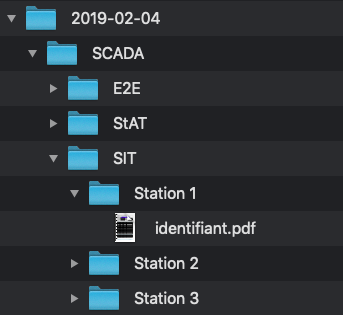
\includegraphics[height=7cm]{ressources/images/figures/tree.png}
\end{center}

\subsubsection{Exportation}

Enfin, les données sous forme de tables étaient exportées au format Excel afin d'être intégrées aux différents outils du projet.

\subsection{Les choix techniques}

Dans cette section, pour chaque étape énoncée précédemment, nous exposerons ainsi les éventuelles difficultés rencontrées pour chacune d'elles, les différentes alternatives techniques possibles et nous justifierons nos choix.

Concernant le langage informatique, j'aurais pus utiliser :
\begin{itemize}
\item \textbf{Node.js :} langage efficace pour extraire des données d'un site web dynamique, mais pas assez stable pour le nombre de requêtes nécessaires à ce projet.
\item \textbf{C ++ :} il propose des performances élevées, mais aurait demandé un investissement horaire démesuré.
\item \textbf{PHP :} ce langage supporte mal le multi-threading et l'ordonnancement de tâches, fonctions pourtant indispensables à ce projet, comme nous le verrons plus bas.
\item \textbf{Python :} c'est l'alternative la plus utilisée pour ce genre de projet, et cela principalement grâce aux bibliothèques surdéveloppées que la communauté Python a mises au point et enrichies.
\end{itemize}

J'ai donc choisi d'utiliser Python. Dans un premier temps j'utilisais Python 2.7, mais la fin de vie de cette version étant annoncée pour janvier 2020 j'ai préféré passer, vers la fin du projet, à Python 3.7.
Ce choix était aussi motivé par la simplicité de cette opération, grâce à l'existence d'un programme nommé \underline{\href{https://docs.python.org/2/library/2to3.html}{2to3}} qui permet de transformer un script écrit en 2.7 en un script compatible 3.7.

\subsubsection{Authentification}

Pour cette partie, j'ai défini une session, avec laquelle j'envoyais une requête de type "post" avec les données nécessaires à l'authentification. Cette requête permettait de simuler la saisie manuelle des données dans les champs dédiés de la page d'authentification puis de simuler l'appui sur le bouton "Se connecter".
Cependant, une autre solution bien plus simple aurait été d'utiliser la clé d'accès à l'\gls{API} de \gls{SnagR} à chaque requête.

En effet, l'outil propose une \gls{API}, qui est une interface donnant accès à certaines de ses fonctions et de ses données, et cela de manière facilitée.

Malheureusement, je n'ai découvert l'existence de cette \gls{API} qu'après avoir réussi à implémenter la méthode d'authentification.

\subsubsection{Extraction des données}

Pour l'extraction des données, j'ai commencé par analyser les différentes requêtes effectuées par \gls{SnagR} et c'est à ce moment-là que j'ai découvert la présence d'une \gls{API} (à travers l'URL d'une requête).

Afin de pouvoir l'exploiter au mieux, j'ai voulu me procurer sa documentation. En explorant l'arborescence du site, j'ai découvert une page contenant une documentation non achevée et obsolète puisqu'elle concernait la version 1 de l'\gls{API} et non la version actuelle (v2).

J'ai donc contacté le service informatique du client (QDVC) puis le service de \gls{SnagR}, mais une telle documentation pour la version 2 ne semblait pas exister.

Il m'a donc fallu comprendre la structure et le fonctionnement de l'\gls{API} par l'expérimentation.
J'ai analysé de nombreuses pages du site jusqu'à obtenir un lot de requêtes suffisant à l'extraction des données nécessaires.

Les réponses à ces requêtes étaient au format JSON, un format de représentation des données.

J'ai donc choisi de générer ces requêtes au sein du script et de récupérer les données résultantes avec un module Python nommé \underline{\href{https://simplejson.readthedocs.io/en/latest/}{simplejson}}.

Le choix de l'extraction des données en deux temps est justifié par deux raisons :
\begin{itemize}
\item Laisser le choix à l'utilisateur des données qu'il veut extraire afin d'actualiser sa base de données.
\item Optimiser le nombre de requêtes exécutées par le script. En effet, une fois la liste des rapports obtenue, au lieu de chercher à extraire les données de tous les rapports, même ceux encore vierges, on ne s'intéresse qu’à ceux qui sont au minimum entamés. Ici nous avons pris comme critère la présence de la signature de l'ingénieur Thales ayant réalisé le test.
\end{itemize}

Toujours dans une démarche d'optimisation de cette étape, j'ai ensuite cherché à réduire le temps d'extraction des données. En effet, il fallait une requête pour pouvoir obtenir les données de chaque \gls{TestCases}, ce qui faisait plus de 15 000 requêtes, plus le temps de traitement de chaque requête.

C'est pour ces raisons qu'initialement, le programme prenait environ une heure à s'exécuter.

C'est ce qui m'a amené à devoir choisir entre le multithreading et le multiprocessing. Ce sont deux techniques d'optimisation dont le principe diffère :
\begin{itemize}
\item Le premier consiste à exécuter des tâches ou fils de tâches (appartenant au même processus) en parallèle tout en utilisant les mêmes ressources (même processeur).
\item Le second consiste à exécuter plusieurs processus en parallèle en utilisant plus de deux processeurs.
\end{itemize}

J'ai choisi le multithreading, car je ne voulais pas concevoir un outil dont les performances dépendraient grandement de la machine qui l'exécute.

À cela j'ai ajouté un système de queue, pour stocker les requêtes en attente d'être exécutées.

Après avoir mis en place cette solution, le temps d'exécution oscillait entre 5 et 10 minutes, car les serveurs du site n'offraient pas une stabilité optimale, ce qui faisait que par moment, plus de 40\% des requêtes échouaient et devaient être effectuées à nouveau.

\subsubsection{Organisation des données}

Pour organiser les données, j'ai utilisé la bibliothèque \underline{\href{https://pandas.pydata.org}{Pandas}} qui est dédiée à l'analyse de données.

La première étape était d'importer les données au format JSON dans des tables. Pour cela j'ai utilisé le module "jsonnormalize" issu de la bibliothèque Pandas.

Cette dernière m'a aussi servie à sélectionner les champs de données que je voulais conserver, filtrer les résultats, joindre des tables et toutes les opérations habituelles lorsqu'on traite avec des tables de données.
Voici ci-dessous les différentes tables que j'ai créées afin de concevoir ma base de données finale.

\newpage
\begin{center}
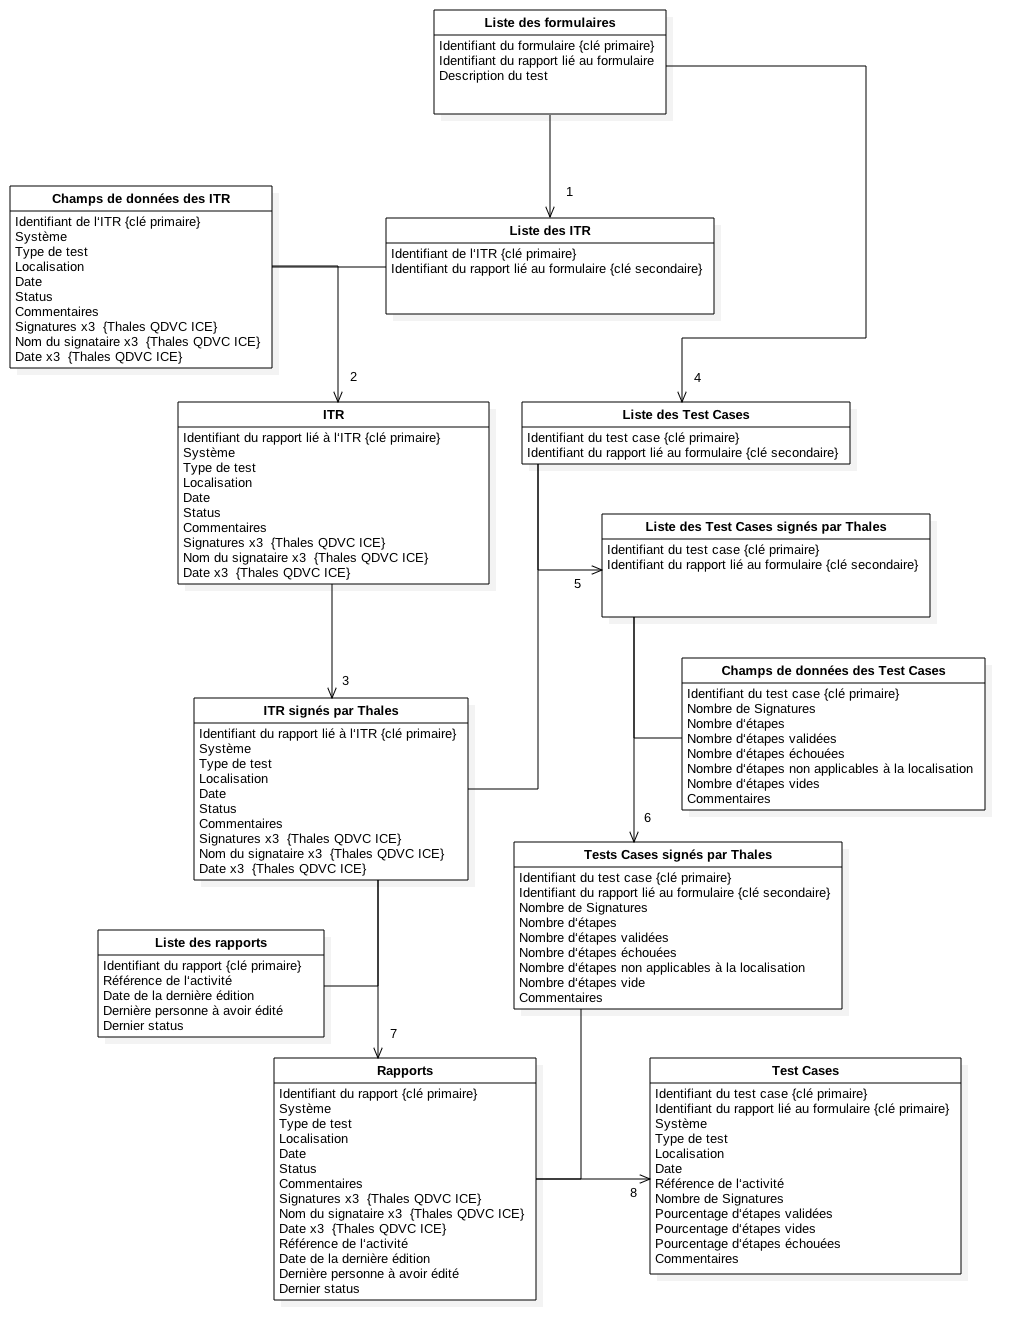
\includegraphics[scale=0.5]{ressources/images/figures/bd.png}
\end{center}
\newpage

Les tables "Listes des formulaire", "Champs de données des ITR", "Champs de données des Test Cases" et "Liste des rapports" sont les tables obtenues en réponse à différentes requêtes envoyées à l'\gls{API} de \gls{SnagR}. 

Les deux tables que l'on cherche à obtenir sont les tables "Rapports" et "Test Cases".

Enfin toutes les autres tables sont des étapes intermédiaires dans l'agencement de ces données.

Voici le détail des différentes opérations réalisées :
\begin{itemize}
\item 1 : on filtre la liste des formulaires en ne retenant que les ITR (première page d'un rapport).
\item 2 : on effectue une jointure des deux tables avec l'identifiant du de l'ITR puis on supprime cet identifiant au profit de l'identifiant du rapport lié à l'ITR qui est aussi unique dont éligible en tant que clé primaire.
\item 3 : on filtre en ne retenant que les ITR signés par Thales.
\item 4 : on filtre en ne retenant que les Tests Cases.
\item 5 : on effectue une jointure des deux tables avec l'identifiant du rapport lié à l'ITR.
\item 6 : on effectue une jointure des deux tables avec l'identifiant du test case.
\item 7 : on effectue une jointure des deux tables avec l'identifiant du rapport lié à l'ITR.
\item 8 : on effectue une jointure des deux tables avec l'identifiant du rapport lié à l'ITR.
\end{itemize}

\subsubsection{Sauvegarde}
Pour cette fonction, j'ai fait le choix de ne télécharger que les rapports au minimum initialisés par Thales. Chaque sauvegarde est stockée dans un dossier ayant pour nom la date de l'exécution en suivant l'arborescence précédemment énoncée.

J'aurais pus faire le choix de ne créer qu'un seul dossier et de ne télécharger que les rapports qui n'avaient pas été encore sauvegardés,
mais le contenu de ces derniers étant dynamique, la seule solution viable était une sauvegarde intégrale et datée à chaque appel de la fonction de sauvegarde.
\subsubsection{Exportation}
Enfin, pour l'exportation, je me suis posé la question du format d'exportation de ces données que je devais choisir.

La solution optimale, selon moi, aurait été d'héberger ce script sur un serveur, l'exécuter en tâche de fond puis créer une interface web pour la consultation et la communication de ces données.

Cependant, cette solution ne correspond pas aux contraintes du projet.

Premièrement, je ne pouvais pas allouer la totalité de mon temps à cette tâche.

Ensuite, le caractère confidentiel de ces données ne me permettait pas de les héberger sur un serveur personnel. Les héberger sur un serveur Thales aurait de toute façon nécessité une validation en interne puis avec le client ainsi qu'un processus assez long (dans le cas où la proposition aurait été acceptée).

%Tout le monde utilise Excel

\newpage
\section{Communication sur l'avancement du projet}

Une fois les données extraites, il faut leur donner un sens afin de pouvoir les exploiter. Sur ce projet, les données issues des rapports étaient indispensables au management ainsi qu'à la communication avec le client. La première étape de cette exploitation est l'analyse des données.

\subsection{Analyse des données}
Si on revient aux raisons qui nous ont poussés à développer l'outil présenté précédemment, une d'entre elles était le manque de cohérence.
En effet, le nombre total de rapports sur \gls{SnagR} étant plus élevé que la réalité, il est, jusque là, impossible de rendre compte de l'avancement, puisque ce dernier s'illustre avec des pourcentages d'accomplissement.

C'est pour cela qu'un travail d'analyse des différentes documentations des systèmes déployés pas Thales a été réalisé avec mon maître de stage ainsi que le manager de l'équipe afin d'obtenir une liste et donc un nombre total des rapports à produire.

Il m'a ensuite fallu m'atteler à la création de différents indicateurs et outils permettant la vérification de la cohérence des données. 

Par exemple, en m'appuyant sur la liste des rapports abordée précédemment, j'ai pu identifier ces rapports sur \gls{SnagR}, ce qui m'a permis d'ajouter de nouveaux filtres afin d'analyser uniquement les 1500 rapports à produire et non les 6000 présents sur \gls{SnagR} (c.f 3.2.1).

Une fois la cohérence des données assurée, je pouvais analyser ces dernières afin d'identifier les données les plus utiles.

Par exemple, en utilisant la date du test ainsi que les dates auxquelles les différents parti ont signé, on allait pouvoir obtenir les délais suivant : 
\begin{itemize}
\item Le délai de remplissage du rapport par Thales (date de signature Thales - date du test)
\item Le délai de signature du rapport par QDVC (date de signature QDVC - date de signature Thales)
\item Le délai de signature du rapport par ICE (date de signature ICE - date de signature QDVC)
\item Le délai total de production du rapport (date de signature ICE - date du test)
\end{itemize}

Une fois les données analysées et les différents problèmes de cohérence résolus, il fallait pouvoir rendre compte de l'avancement à l'équipe Thales.

\subsection{Communication interne}
Avoir choisit comme format de donnée un fichier Excel présente l'avantage de pouvoir facilement transmettre les données et de pouvoir réaliser des indicateurs d'avancement modulables.

Les indicateurs nécessaires diffèrent en fonction de leur destinataire, et à la vue du nombre important de membres sur le projet, il a fallu réaliser un nombre important de graphiques utilisant les données précédemment exportées. 

En voici quelques un :

\begin{itemize}
\item Sur une même figure : l'histogramme retraçant la production de rapport journalière, la courbe d'évolution du nombre total de rapports produits, la courbe correspondant à l'avancement programmé ainsi qu'une courbe de tendance prévoyant l'évolution à venir du nombre total de rapports produits, basée sur l'avancement durant les deux semaines précédentes.
\item Un tableau croisé dynamique permettant de connaitre le statut de complétion des \gls{TestCases} liés à des exigences sécurité pour chaque localisation où ils sont applicables.
\item Un tableau croisé dynamique permettant de connaitre l'état d'avancement des rapport de chaque système en fonction de chaque localisation où le système est présent.
\item Des histogrammes illustrant le nombre de rapport produit par rapport au nombre de rapport restant en fonction de différents filtres, critères (par système, par type de test etc)
\item Un diagramme représentant, en fonction du délai total de production moyen, la part de responsabilité des différents partis (Thales, QDVC, ICE) dans ce délais.
\end{itemize}

De plus, puisque je n'étais pas le seul à communiquer un rapport d'avancement, il fallait s'assurer de la cohérence entre les différents rapports envoyés par l'équipe \gls{TC}.

Les deux autres rapports principaux étaient le rapport du manager de l'équipe gestion de projet et celui du manager de l'équipe \gls{TC}.

Le premier était un rapport tenant compte du planning annoncé et proposant une estimation officielle de l'avancement planifié au cours des semaines suivante.

Le second était un rapport de l'avancement des test, et non de l'avancement de la production des rapports. Il était donc utile de croiser nos données pour identifier les tests déjà effectués mais pour lesquels aucuns rapports n'avaient été produit. 
Cela nous permettait d'identifier les points bloquants avant de reporter l'avancement au client.

Ces deux rapports utilisant le découpage en activités (c.f 3.2.1) et non le découpage en rapport, contrairement à moi, il me fallu réaliser une table de correspondance entre les noms des activités et les noms des rapports, afin de pouvoir lier et comparer ces trois fichiers.

Une fois que ces 3 rapports faisaient état du même avancement, nous le communiquions au client.


\subsection{Communication avec le client}

%Organisation des données et des indicateurs pour correspondre aux différents scopes proposés par l'équipe RAMS (Pilot, Safety Strategy et Safety Related)
La communication avec le client doit se faire certes en toute transparence, mais au vue de l'expertise métier détenue par Thales, cette communication de l'avancement se doit d'être structurée autours d'objectifs. 

C'est pour cette raison que l'équipe \gls{RAMS} a proposé de présenter les données autours de 4 objectifs :
\begin{itemize}
\item \textbf{1. Pilot :} on met en priorité 1 (maximale) certains rapports de manière à pouvoir prouver la conformité du système à chaque exigence sécurité dans au moins une localisation, en essayant, dans la mesure du possible, de réduire le nombre de stations concernées afin de pouvoir y organiser des visites de démonstration de leur conformité en terme de sécurité. 
\item \textbf{2. Stratégie SIL :} ici la stratégie reste la même pour les exigences \gls{SIL}0 (c.f 3.1.1), on inclut les mêmes localisation que pour l'objectif Pilot. Cependant pour les exigences \gls{SIL}2, on intègre au spectre de cet objectif toutes les localisations ou elles sont applicables.
\item \textbf{3. Sécurité :} ensuite l'objectif est la conformité des toutes les localisations du projet avec les exigences sécurité y étant applicables.
\item \textbf{4. Général :} enfin l'objectif est la conformité des toutes les localisations du projet avec toutes les exigences y étant applicables.
\end{itemize}


Les différents indicateurs exposés dans la partie précédente ont du tenir compte de ces objectifs, ainsi, dans mon rapport hebdomadaire que j'envoyais à l'équipe Thales ainsi qu'au client, je fournissais des indicateurs d'avancement pour chaque objectif, en mettant l'accent sur l'objectif le plus prioritaire à l'instant t.


%Blockers externes
La communication avec le client, bien que basée sur les mêmes données, imposait un niveau de détails plus important, pour, par exemple, être capable de justifier d'éventuels délais.

Ainsi nous ajoutions des commentaires, des observations à certains des indicateurs pour proposer une certaine lecture des données au client. 
%Difficultés personnelles rencontrées face au client (dues à une première expérience)
Il est important de rappeler ici que Thales est sur ce projet en tant que prestataire de QDVC et ne fait donc pas partie du Consortium.
Pourtant sur tout les systèmes \gls{CCS}, qui représentent une partie très importante des différents systèmes du projet, c'est Thales qui possède l'expertise métier. 

De plus, le client était dans les mêmes locaux que Thales, ce qui compliquait parfois la préservation des informations confidentielles. 

Ainsi différents facteurs pouvaient compliquer la communication avec le client, d'où l'importance cruciale de savoir identifier si les points bloquants avaient des causes internes (due à l'équipe \gls{TC}, Installation ou offshore) ou bien externes (due aux autres prestataires, au client, au génie civil, à Alstom).

%QQchose

\newpage
\section{Formation et transmission}

Durant ce stage, j'ai du former des membres du projet de manière ponctuelle mais aussi de manière continue.
\subsection{Sensibilisation des membres de l'équipe }


Comme nous l'avons vu précédemment, il pouvait arriver que certains rapports de test restent vide même une fois le test réalisé. Cela pouvait se produire pour plusieurs raisons : 
\begin{itemize}
\item Un simple oubli de la part de l'ingénieur Thales responsable du test. Dans ce cas, un simple rappel suffisait.
\item Un mauvaise communication au sujet du caractère prioritaire de la production des rapports. Ici la solution choisi par le management était d'afficher les indicateurs que je produisait dans l'open space de l'équipe \gls{TC} afin que tout le monde soit en phase avec les objectifs fixés.
\item Une charge de travail trop importante en terme de test, ce qui rends impossible la production des rapports correspondant à ces tests. La seule solution ici était d'en référer au management afin de répartir à nouveau les ressources pour libérer l'ingénieur en question.
\end{itemize}

%absence validation données
Mais le problème majeur auquel j'ai du faire face est celui des données renseignées par les membres du projet (pas uniquement Thales mais aussi QDVC et ICE).

En effet, l'interface d'édition de rapports que propose \gls{SnagR} présente un important défaut : elle n'a pas été dotée d'une fonction de validation des données.

C'est un problème majeur car des données erronées viennent fausser les indicateurs produits et menacent la cohérence de la base de données.

La solution me paraissant la plus robuste était de produire une documentation à l'attention de tous les utilisateurs de \gls{SnagR} à même de remplir des rapports. 
Dans cette documentation j'ai énoncé une dizaine de règles à respecter, illustrées par des exemples et captures d'écran du site. 

À la fin de cette documentation j'ai ajouté une convention de nommage concernant 3 champs de données : la localisation, le système et le type de test. 
Sans cette démarche, les données n'auraient jamais le même format puisqu'il y autant de façon de les renseigner qu'il y a d'utilisateurs.

En plus de distribuer cette documentation par mail à tout le projet, j'ai organisé une petite formation pour énoncer clairement ces règles et répondre à toutes les question des utilisateurs durant la même séance.

%Listing ?
Nous avons parlé ici de petites formations ponctuelles, mais au cours de mon dernier mois, j'ai du former quelqu'un en continu.

\newpage
\subsection{Tuilage}

À la fin de mon stage, j'ai eu la chance de connaitre mon remplaçant un mois à l'avance. Le but de cette section est de retracer chronologiquement les différentes étapes de ce tuilage.

\begin{itemize}
\item Tout d'abord, progressivement au cours du stage j'ai rédigé une documentation sur le script Python tout en le commentant. Je me suis imposé cette pratique car d'expérience je sais à quel point il est complexe de revenir sur des lignes de code écrites auparavant, et je ne voulais pas avoir à subir cette tâche laborieuse à la fin de mon stage.
\item Dans un second temps,  mon maître de stage m'a demandé de lui fournir un profil type pour mon remplaçant. Au bout d'un peu plus de 4 mois de stage, on m'avait proposé de continuer a sein du projet après mon stage, mais la date limite de dépôt de dossier de candidature pour une césure en P19 était déjà passée.
\item Tutoriel vidéo réalisé pour mon remplaçant.
\item Délégation du travail progressive
\item État de l'avancement (pending tasks, pending issues).
\end{itemize}





